%%%%%%%%%%%%%%%%%%%%%%%%%%%%%%%%%%%%%%%%

\begin{edXchapter}{Matrix}

\begin{edXsection}{ProblemSet1}

\begin{edXvertical}

% Question 1
\begin{edXproblem}{Question1}
역행렬이 존재하는 두 행렬 $A$와$B$가
$A = \left( \begin{array}{cc}
5 & 2 \\
7 & 3 \\
\end{array} \right)  B$ 를 만족시킬 때, 행렬 $AB^{-1}+BA^{-1}$의 모든 성분의 합을 구하여라.
\begin{figure}
	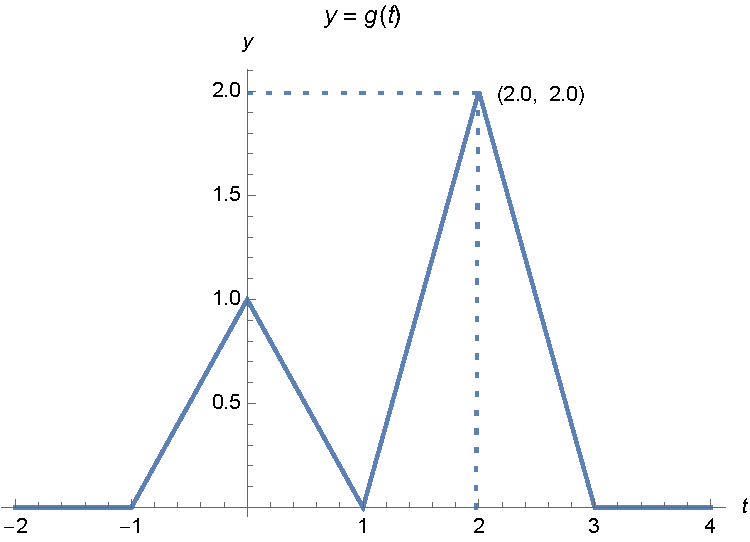
\includegraphics[width=0.4\textwidth, left]{2015midtermPractice2-figure1.pdf}
\end{figure}

% Question 1 Answer Box
\edXabox{expect="16" type="numerical"}

% Question 1 Solution
\begin{edXsolution}
$\left( \begin{array}{cc}
	5 & 2 \\
	7 & 3 \\
\end{array} \right)=C$라고 하자.\\
조건식의 양변에 $B^{-1}$을 곱하면
\begin{equation}
 AB^{-1}=CBB^{-1}=C 
\end{equation}
조건식의 양변에 $A^{-1}$을 곱하면\\
$AA^{-1}=CBA^{-1}$이므로\\
\begin{equation}
E=CBA^{-1}
\end{equation}
(2)의 양변에 $C^{-1}$을 곱하면\\
\begin{equation}
C^{-1}=C^{-1}CBA^{-1}=BA^{-1}
\end{equation}
(1)(3)에서 $AB^{-1}+BA^{-1}=C+C^{-1}=\left( \begin{array}{cc}
5 & 2 \\
7 & 3 \\
\end{array} \right)+\left( \begin{array}{cc}
3 & -2 \\
-7 & 5 \\
\end{array} \right)=\left( \begin{array}{cc}
8 & 0 \\
0 & 8 \\
\end{array} \right)$\\
그러므로 $AB^{-1}+BA^{-1}$의 모든 성분의 합은 $16$
\begin{figure}
	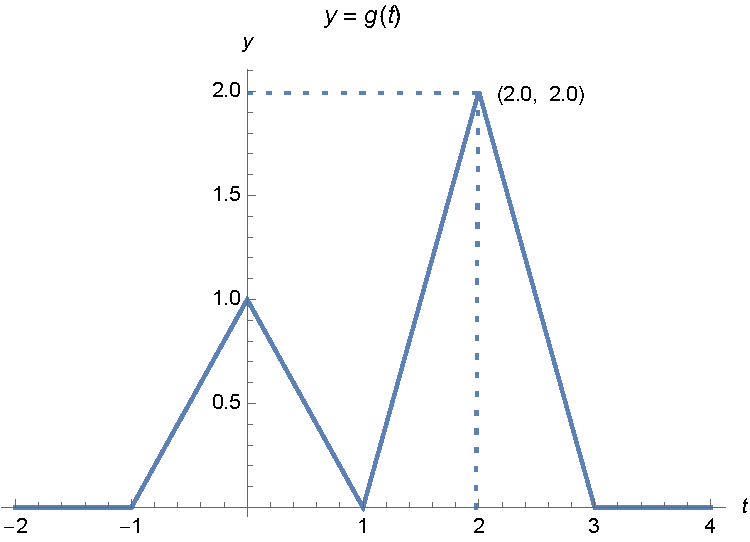
\includegraphics[width=0.4\textwidth, left]{2015midtermPractice2-figure1.pdf}
\end{figure}

\end{edXsolution}

\end{edXproblem}

% Question 2
\begin{edXproblem}{Question2}

$a = \sqrt{2}$, $b = \sqrt[3]{3}$을 $a$, $b$로 나타낸 것은?

\edXabox{type="multichoice" expect="Yellows" options="Red", "Green", "Yellow", "Blue"
}


\end{edXProblem}
%%%%%%%%%%%%%%%%%%%%%%%%%%%%%%%%%%%%%%%%

\end{edXvertical}

\end{edXsection}

\end{edXchapter}
